\documentclass[12pt]{article}

\usepackage[margin=1in]{geometry}
\usepackage{fancyhdr}
\usepackage{graphicx}
\usepackage{setspace}
\usepackage{titlesec}
\usepackage{enumitem}
\usepackage{longtable, booktabs}

%---------------------------------------------------------------------------------
% Section Formatting (optional: smaller spacing before sections)
%---------------------------------------------------------------------------------
\titlespacing\section{0pt}{*2}{*1}
\titlespacing\subsection{0pt}{*1.5}{*0.8}
\titlespacing\subsubsection{0pt}{*1.2}{*0.5}

%---------------------------------------------------------------------------------
% Cover Page
%---------------------------------------------------------------------------------
\pagestyle{fancy}
\fancyhf{}
\fancyhead[L]{USC Facilities: Rain Barrel Water Pump System}
\fancyfoot[C]{\thepage}

\begin{document}
\onehalfspacing

\title{
    \vspace{2in}
    \textbf{EMCH428-002} \\[1ex]
    \textbf{DFX Report} \\[1ex]
    \textbf{Sponsor: USC Facilities} \\[1ex]
    \vspace{2in}
}

\author{
    \textbf{Team Members:} \\[2ex]
    Tanner Harmon\\[1ex]
    Presston McConnell\\[1ex]
    William Wenzel\\[1ex]
    Jacob Vaughn\\[2ex]
}

\date{}

\maketitle
\thispagestyle{fancy}

\newpage

\setcounter{page}{2} % Start page numbering from the second page

%---------------------------------------------------------------------------------
% 1. Design Refinement Introduction
%---------------------------------------------------------------------------------
\section{Design Refinement Introduction}
\begin{itemize}[leftmargin=1.5cm]
    \item The purpose of this report is to present the final design refinements applied to the rain barrel water pump system.
    \item Parameters considered for refinement include:
    \begin{itemize}
        \item Manufacturability and Assemblability (single-use product focus)
        \item Cost
        \item Safety
        \item Energy usage
        \item Material selection
    \end{itemize}
    \item Key optimization outcomes:
    \begin{itemize}
        \item Reduced complexity of the enclosure for simpler assembly
        \item Improved pump and piping arrangement for better flow and pressure
        \item Lowered material costs through part reduction
        \item Enhanced safety features and instructions to reduce user risk
    \end{itemize}
    \item Recommendations for future builds:
    \begin{itemize}
        \item Incorporation of a real-time water usage monitor
        \item Additional insulation for extreme temperature conditions
        \item Use of standardized fittings to maintain cost savings
    \end{itemize}
\end{itemize}


%---------------------------------------------------------------------------------
% 2. Design for Manufacturability and Assembly
%---------------------------------------------------------------------------------
\section{Design for Manufacturability and Assembly}
\begin{itemize}[leftmargin=1.5cm]
    \item Key manufacturing optimization principles:
    \begin{itemize}
        \item Material selection (plywood panels instead of multiple plank boards)
        \item Component selection (standard pumps, valves, and fittings)
        \item Poka-yoke (labeled wiring and standard connection points)
        \item Part reduction (minimizing extra fasteners and brackets)
    \end{itemize}
\begin{figure}[h!]
    \centering
    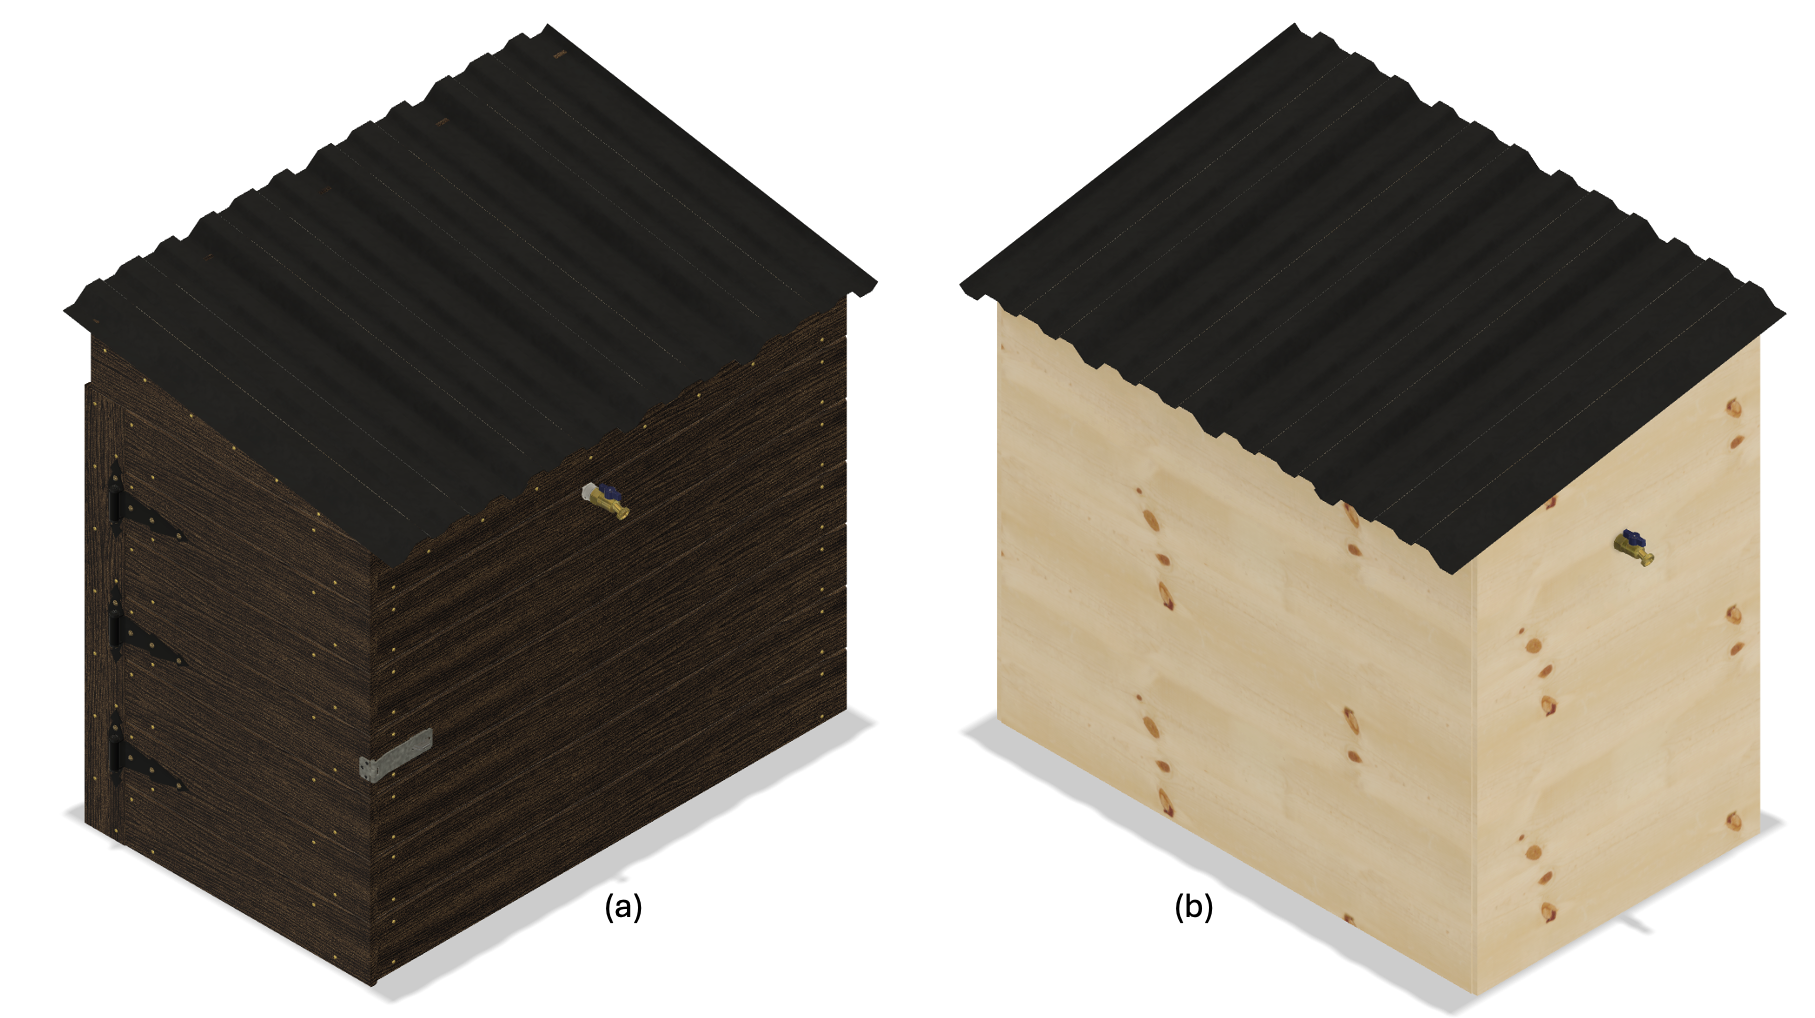
\includegraphics[width=\linewidth]{before_after.png}
    \caption{Before and After Assembly Refinements}
    \label{fig:before_after}
\end{figure}
    \item Refinement actions:
    \begin{itemize}
        \item The number of fasteners at each corner was reduced by increasing the spacing between them compared to the original design.
        \item Prefabricated plywood panels replaced multiple deck planks, reducing assembly time.
        \item Clear labeling of piping parts to avoid reversed installation.
    \end{itemize}
    
    \item Tradeoffs encountered:
    \begin{itemize}
        \item Slightly higher plywood cost was accepted in order to reduce labor and part count.
        \item Slight increase in enclosure footprint allowed for easier internal access and fewer awkward joins.
    \end{itemize}
\end{itemize}




%---------------------------------------------------------------------------------
% 3. Design for Cost
%---------------------------------------------------------------------------------
\section{Design for Cost}
\begin{itemize}[leftmargin=1.5cm]
    \item Design cost considerations:
    \begin{itemize}
        \item Manufacturing process (selecting methods requiring minimal specialized tools)
        \item Material selection (use of standard PVC fittings and plywood for cost control)
        \item Bulk orders and standardization (fewer unique part types)
        \item Product robustness and maintainability to reduce long-term costs
    \end{itemize}

    \item Specific cost-related features:
    \begin{itemize}
        \item Bulk purchase of fasteners resulted in lower unit cost.
        \item Consistent pipe diameter minimized the variety of elbows and tees.
        \item Replacing multiple small boards with larger panels reduced labor hours.
    \end{itemize}

    \item Recommendations for future cost savings:
    \begin{itemize}
        \item Further exploration of alternative materials (e.g., recycled composites).
        \item Negotiation with suppliers to obtain discounts when multiple units are produced.
        \item Potential reuse of some components (pump or pressure tank) if the design is disassembled.
    \end{itemize}
\end{itemize}


%---------------------------------------------------------------------------------
% 4. Design for Safety
%---------------------------------------------------------------------------------
\section{Design for Safety}

\subsection{Identified Hazards}
\begin{enumerate}[leftmargin=1.5cm]
  \item \textbf{Splintering and sharp edges} on raw‐wood panels  
  \item \textbf{Electrical shock} from external pump wiring or exposed conductors  
  \item \textbf{Over‐pressurization} of plumbing or hose connections leading to blow‐off  
  \item \textbf{Pinch points} between the hinged lid and side panels  
  \item \textbf{Slippery surfaces} due to water spills, condensation, or algae growth  
  \item \textbf{Tripping hazards} around the unit footprint and hose runs  
  \item \textbf{Surface overheating} of exterior panels in direct sunlight  
  \item \textbf{Leakage} at the faucet–valve interface under sustained pressure  
\end{enumerate}

\subsection{Health \& Safety Solutions}
\begin{table}[h!]
    \centering
    \caption{Health \& Safety Mitigations for Identified Hazards}
    \label{tab:safety_mitigations}
    \begin{tabular}{l p{0.65\textwidth}}
    \hline
    \textbf{Hazard} & \textbf{Mitigation / Design Solution} \\
    \hline
    Splintering \& sharp edges  
      & All exterior edges chamfered and sanded to 120-grit; surfaces sealed with food-safe mineral oil. \\

    Electrical shock  
      & GFCI-protected circuit, sealed cable glands, cord strain relief, and IP65-rated junction enclosure. \\

    Over-pressurization  
      & 1.5 bar pressure-switch cutoff and 2 bar relief valve; assemblies pressure-tested to 2.5 bar before shipping. \\

    Pinch points  
      & Integrated finger-recess catches and inset bump stops to prevent full-force closure. \\

    Slippery surfaces  
      & Built-in drain channels under drip trays; anti-microbial surface finish to inhibit algae. \\

    Tripping hazards  
      & Low-profile hose routing clips; optional anti-slip floor mat with anchor points. \\

    Surface overheating  
      & Two 10 mm × 100 mm ventilation slots per long panel; UV-reflective clear coat optional. \\

    Leakage at valve  
      & EPDM gasket seals; torque-limited blue-knob valve; each unit tested at 2 bar for 1 hour. \\
    \hline
    \end{tabular}
\end{table}

\subsection{Recommendations \& Warnings}
\begin{itemize}[leftmargin=1.5cm]
  \item \textbf{Winterization:} Drain all water, insulate exposed hoses, and store indoors if ambient $<0\,^\circ\mathrm{C}$.  
  \item \textbf{Routine Inspection:} Monthly checks of hoses, gaskets, wiring, and hinge mechanisms; replace any worn or corroded parts.  
  \item \textbf{User Cautions:} Do not disassemble pressurized components; avoid contact with panels after extended sun exposure.  
  \item \textbf{Maintenance:}
    \begin{itemize}
      \item Tighten valve fittings to specified torque (3 Nm) quarterly.  
      \item Re-apply mineral oil seal annually or after heavy use.  
      \item Clean ventilation slots of debris at least twice per year.  
    \end{itemize}
  \item \textbf{Emergency Procedures:} In case of leak or electrical fault, turn off main power via GFCI, depressurize system using relief valve, then contact qualified service personnel.  
\end{itemize}


%---------------------------------------------------------------------------------
% 5. Design for Customer Requirements
%---------------------------------------------------------------------------------
\section{Design for Customer Requirements}
\begin{itemize}[leftmargin=1.5cm]
    \item \textbf{Product Mission:}  
    A system that delivers rainwater efficiently and reliably for garden irrigation while reducing manual effort and aligning with the sponsor's sustainability goals.

    \item Customer needs, requirements, and metrics:
    \begin{itemize}
        \item Needs and parameters were mapped in a Metrics Matrix to confirm flow rate, pressure, cost, and usability.
        \item Please refer to Chapter 2 and 3 for the Complete Metrics Matrix.
    \end{itemize}


    \item \textbf{Product-Parameter Refinement:}  
    Table~\ref{tab:parameter_refinement} details each key parameter’s original and refined values along with the rationale for change.

\begin{table}[h!]
  \centering
  \caption{Refined Product Parameters (Before vs.\ After)}
  \label{tab:parameter_refinement}
  % scale to full text width
  \resizebox{\textwidth}{!}{%
    \begin{tabular}{p{3cm} p{2cm} p{2cm} p{8cm}}
      \hline
      \textbf{Parameter}       & \textbf{Original}      & \textbf{Refined}           & \textbf{Rationale}                                                   \\
      \hline
      Wall thickness           & 12 mm                  & 15 mm                      & +25 \% stiffness to limit deflection under 50 N load                   \\
      Joint clearance          & 0.2 mm                 & 1.0 mm                     & Wider clearance eases board fit-up and reduces assembly time           \\
      Panel size               & 500 × 300 mm           & 600 × 400 mm               & Fewer panels → fewer joints → faster assembly                         \\
      Material grade           & Standard pine (C)      & Knotty pine (B)            & Improved strength and appearance at minimal cost increase             \\
      Fastening scheme         & 4 ext.\ screws/joint   & 2 screws + biscuit joints  & Eliminates exterior holes; zero visible fasteners                     \\
      Ventilation slots        & None                   & 2×(10×100 mm) per panel    & Provides passive cooling to keep surface < 40 °C                       \\
      Edge chamfer             & 0°                      & 45° at 2 mm                & Removes sharp edges to eliminate splinter risk                        \\
      Gasket thickness         & 1 mm                   & 2.5 mm                     & Thicker seal to ensure < 0.1 L/h leakage under 1 bar                 \\
      Valve torque spec        & N/A                    & 3 Nm ± 0.2 Nm              & Consistent manual operation without overtightening                   \\
      Assembly time            & 45 min                 & 25 min                     & Simplified joinery and fewer fasteners halve construction time        \\
      Unit weight              & 4.2 kg                 & 3.4 kg                     & Lighter panels and reduced hardware improve portability              \\
      Unit cost                & \$75                   & \$48                       & Material and hardware optimization achieves < \$50 target            \\
      Coating finish thickness & 0 (raw)                & 0.1 mm mineral oil layer   & Food-safe seal without altering appearance                          \\
      Hinge type               & Strap hinge            & Concealed piano hinge      & Hidden hinge reduces exposed hardware count                          \\
      Drip channel depth       & None                   & 3 mm                       & Prevents standing water near valve to reduce slip hazard             \\
      \hline
    \end{tabular}
  }
\end{table}


\subsection{Design for Pressure and Flow}
\begin{itemize}[leftmargin=1.5cm]
    \item Parameter considered: Reliable irrigation coverage.
    \item Relevant refinements:
    \begin{itemize}
        \item Larger pressure tank and high-pressure switch were added to stabilize flow.
        \item Fewer pipe diameter changes minimized friction losses.
    \end{itemize}
    \item Recommendations and tradeoffs:
    \begin{itemize}
        \item A small increase in upfront cost was necessary to purchase the pressure tank.
        \item Substantial improvement in user satisfaction and watering efficiency justified the extra cost.
    \end{itemize}
\end{itemize}

\subsection{Design for Assembly Ease}
\begin{itemize}[leftmargin=1.5cm]
    \item Parameter considered: Minimized assembly time and error risk.
    \item Relevant refinements:
    \begin{itemize}
        \item Labeled connections on pump, tank, and piping.
        \item One-piece plywood panels rather than multiple smaller boards.
    \end{itemize}
    \item Recommendations and tradeoffs:
    \begin{itemize}
        \item Marginally higher cost for larger plywood sheets balanced by savings in labor.
        \item Reduced overall assembly error rates from fewer alignment issues.
    \end{itemize}
\end{itemize}


%---------------------------------------------------------------------------------
% 6. Conclusions and Recommendations
%---------------------------------------------------------------------------------
\section{Conclusions and Recommendations}
\begin{itemize}[leftmargin=1.5cm]
    \item \textbf{Key refinements and changes}:
    \begin{itemize}
        \item Part count reduction in the enclosure
        \item Standardized 3/4'' PVC fittings
        \item Simplified pump layout for improved performance
        \item GFCI and relief valve for improved safety
    \end{itemize}

    \item \textbf{Future recommendations}:
    \begin{itemize}
        \item Adding a flow sensor or digital pressure gauge for better monitoring
        \item Exploring modular insulation panels for winterization
        \item Investigating solar panel or battery upgrades to reduce operating costs
    \end{itemize}

    \item \textbf{Tradeoffs and compromises}:
    \begin{itemize}
        \item Increased enclosure footprint for easier maintenance
        \item Slightly higher plywood cost chosen over complex multi-board assembly
        \item Limited automation to remain within budget constraints
    \end{itemize}
\end{itemize}

\end{document}
